\documentclass{beamer}
\usepackage{graphicx}

\usepackage[utf8]{inputenc}
\usepackage[T1]{fontenc} 

\usetheme[hideallsubsections]{PaloAlto}

%\usepackage{tikz}
\usepackage{verbatim}
\usepackage{tabularx}
\usepackage{array}

% vertically centering in tables when X
\renewcommand{\tabularxcolumn}[1]{>{\small}m{#1}}
\usepackage{makecell}
\usepackage{color}
\usepackage{diagbox}

\usepackage[english]{babel}
\usepackage{lmodern} 


% \setbeamertemplate{sections in toc}[sections numbered]
% \usetikzlibrary{arrows,shadows,shapes,backgrounds,positioning}
% \beamertemplatetransparentcovered

% insert page number in Beamer Navigation Bars
\addtobeamertemplate{navigation symbols}{}{%
    \usebeamerfont{footline}%
    \usebeamercolor[fg]{footline}%
    \hspace{1em}%
    \insertframenumber/\inserttotalframenumber
}

% set head height
\makeatletter
\setlength{\beamer@headheight}{0.7cm}
\makeatother


\title[]{Logiciels libres} 
\author{Rémi Boulle}
\date{}       
\institute{}        

\begin{document}

% section titles in a special slide
\AtBeginSection[]{
  \begin{frame}
    \vfill \centering
    \begin{beamercolorbox}[sep=8pt,center,shadow=true,rounded=true]{title}
      \usebeamerfont{title}\insertsectionhead\par%
    \end{beamercolorbox}
    \vfill
  \end{frame}
}

%%%%%%%%%%%%%%%%
% Title
%%%%%%%%%%%%%%%%

\begin{frame}
  \titlepage
\end{frame}

%%%%%%%%%%%%%%%%%%%%%%%%%%%%%%%%%%%%%%%%%%%%%%%%%%%%%%%%
% Examples of free software Notepad-plus-plus and ffmpeg
%%%%%%%%%%%%%%%%%%%%%%%%%%%%%%%%%%%%%%%%%%%%%%%%%%%%%%%%

\section{Exemples}

\setbeamertemplate{background canvas}{\centering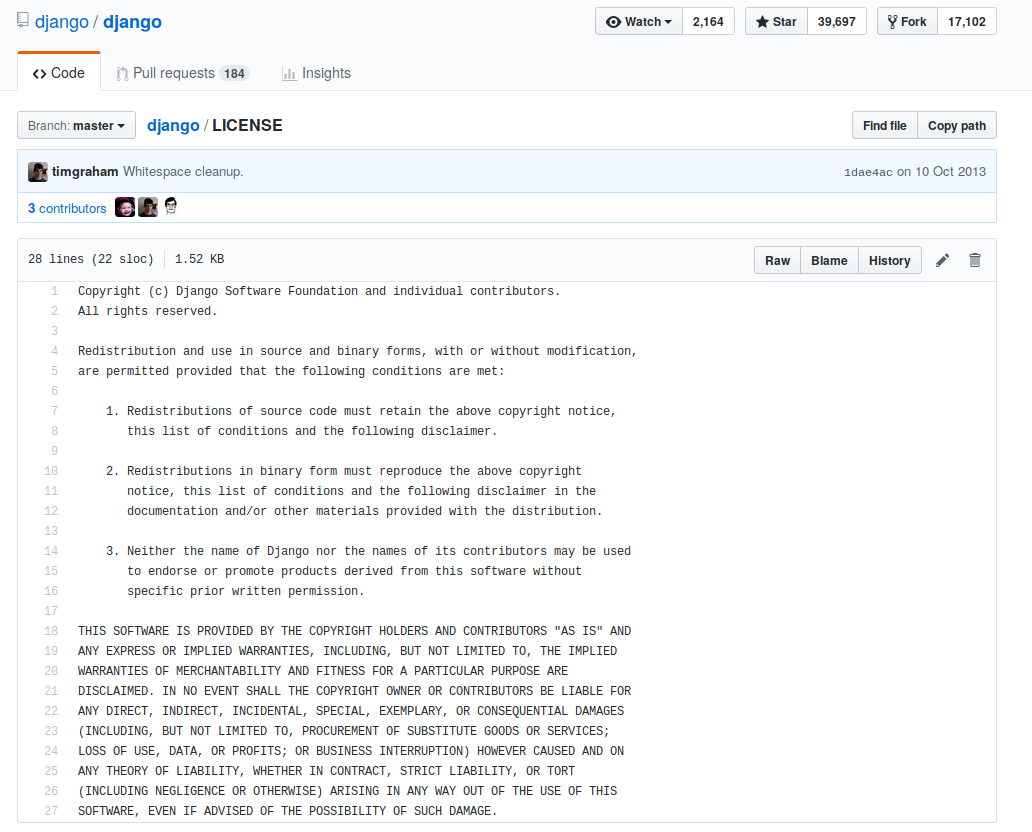
\includegraphics
  [width=\paperwidth]{images/django-licence-screenshot.png}}
\begin{frame}[plain]%{RMS}
%  
\end{frame}
\setbeamertemplate{background canvas}{}

\setbeamertemplate{background canvas}{\centering\includegraphics
  [width=\paperwidth]{images/notepad-plus-plus-LICENSE.jpg}}
\begin{frame}[plain]%{RMS}
%  
\end{frame}
\setbeamertemplate{background canvas}{}

\setbeamertemplate{background canvas}{\centering\includegraphics
  [width=\paperwidth]{images/notepad-plus-plus-scancode.jpg}}
\begin{frame}[plain]%{RMS}
%  
\end{frame}
\setbeamertemplate{background canvas}{}


\setbeamertemplate{background canvas}{\centering\includegraphics
  [width=\paperwidth]{images/scancode-ffmpeg.png}}
\begin{frame}[plain]%{RMS}
%  
  \note{RMS}
\end{frame}
\setbeamertemplate{background canvas}{}

\setbeamertemplate{background canvas}{\centering\includegraphics
  [width=\paperwidth]{images/FFmpeg-license-and-legal-consideration.jpg}}
\begin{frame}[plain]%{RMS}
%  
  \note{RMS}
\end{frame}
\setbeamertemplate{background canvas}{}

\begin{frame}{Pourquoi est-ce important ?}
  \begin{alertblock}{Pourquoi est-ce important ?}
    \begin{itemize}
    \item Il est rare d'écrire un logiciel \emph{from scratch...}
    \item Un gros projet informatique réutilise souvent du code
      tiers...
    \item La qualité du code est souvent meilleure...
    \item En tant que futur ou future "pro", il est de votre
      devoir/responsabilité de savoir de quoi il est question !
    \end{itemize}


  \end{alertblock}

  Les résultats d'audits sont parfois surprenants... Vos avis ?

\end{frame}



%%%%%%%%%%%%%%%%%%%%%%%%%%%%%%%%%%%%%%%%%%%%%%%%%%%%%%%%
% Context, vocabulary
%%%%%%%%%%%%%%%%%%%%%%%%%%%%%%%%%%%%%%%%%%%%%%%%%%%%%%%%

\section{Contexte}

\begin{frame}{D'où cela vient-il ?}
  \begin{itemize}
  \item projet GNU en 1984 par Richard Stallman (RMS)
  \item Première GPL : 25 février 1989
  \item la technique est un moyen pour atteindre un but social
  \item 1991 : Système d'exploitation inspiré de Minix (\textit{« just
      a hobby, won’t be big and professional like gnu »}) par Linus
    Torvalds.
  \item 1993 : création de Red Hat (au Nasdaq en 1999), licence Apache
  \item 1998 : libération de Netscape
  \item 1998 : fracture entre « libre » et « open-source » (OSI)
    autour du \textit{copyleft} par Éric Raymond.
  \end{itemize}
\end{frame}



\setbeamertemplate{background canvas}{\centering\includegraphics
  [width=\paperwidth]{images/rms.jpg}}
\begin{frame}[plain]%{RMS}
%  
  \note{RMS}
\end{frame}



\setbeamertemplate{background canvas}{\centering\includegraphics
  [height=\paperheight]{images/LinusTorvalds.jpg}}
\begin{frame}[plain]%{LT}
%  
  \note{Linus Torvalds}
\end{frame}
\setbeamertemplate{background canvas}{}



\begin{frame}{Communautés et structures du libre}

  \begin{block}{International}
    Free Software Fondation : \url{https://www.fsf.org/}

    Open Source Initiative : \url{https://opensource.org/}

    Linux Fondation : \url{https://www.linuxfoundation.org/}

    Communautés de développeurs par projets (debian, Django, d3js,
    python, ubuntu...)
  \end{block}

  \pause

  \begin{block}{France}
    CNLL : \url{http://cnll.fr/}

    April : \url{https://april.org/}

    Framasoft : \url{https://framasoft.org/}

    Toulibre : \url{http://toulibre.org/}

    etc...
  \end{block}
\end{frame}


\begin{frame}{Libre et/ou Opensource}

  \begin{block}{Libre}
    Mouvement social, question de liberté et de
    communauté. \textit{"Toutes les libertés dépendent de la liberté
      informatique, elle n’est pas plus importante que les autres
      libertés fondamentales mais, au fur et à mesure que les
      pratiques de la vie basculent sur l’ordinateur, on en aura
      besoin pour maintenir les autres libertés". (RMS)}
  \end{block}

  \begin{block}{Open-source}
    Open-source : code ouvert, méthodologie de développement,
    \textit{"l'idéologie, c'est nul"} (selon LT), pragmatisme
  \end{block}

  On est toujours l'idéologue de quelqu'un... Débat dépassé ?
\end{frame}


\section{Vocabulaire}

\begin{frame}{Vocabulaire}

  \begin{itemize}
  \item \textbf{Logiciels privatifs} aussi dits \textbf{propriétaires}
    mais tous le sont... ou \textbf{logiciels privateurs} car
    limitent, \textbf{par choix}, vos libertés.
  \item \textbf{Copyleft} : \textit{droit laissé}, obligation de
    garantir que les libertés offertes par la licence soient
    préservées lors de la redistribution.
  \item \textbf{Copyright} : pas de valeur juridique particulière en
    France mais permet d'identifier les auteurs.
  \item Oeuvre : création originale empreinte de la personnalité de
    l'auteur. Plutot \textbf{création intellectuelle} dans le monde
    numérique.
  \item \textbf{Industrie du logiciel} : selon le PE, industrie est
    "automated production of material goods"...
  \end{itemize}
\end{frame}


\setbeamertemplate{background
  canvas}{\hspace{1.5cm}\centering\includegraphics%[scale=0.5]{images/Copyright.png}}
  [height=\paperheight]{images/Copyright.png}}
\begin{frame}[plain]%{LT}
%  
\end{frame}
\setbeamertemplate{background canvas}{}

\begin{frame}{Droit d'auteur}

  \begin{itemize}
  \item Droits patrimoniaux
    \begin{itemize}
    \item Droit de reproduction, de représentation
    \item Droit de suite (pas pour les logiciels)
    \item Droits voisins
    \end{itemize}
  \item Droits extra-patrimoniaux
    \begin{itemize}
    \item perpétuels et inaliénables
    \item paternité, divulgation respect de l'oeuvre, repentir,
      retrait (quasi éradication dans le numérique).
    \end{itemize}
  \end{itemize}

 \begin{alertblock}{Droit d'auteur adapté}
   Libre et privatif sont régis par le \textit{droit d'auteur adaptés
     au logiciels}.
 \end{alertblock}

  \begin{alertblock}{Gauche d'auteur}
    Le libre est adossé au droit d'auteur.
  \end{alertblock}
  
  Les idées sont de libre parcours.
\end{frame}


\setbeamertemplate{background
  canvas}{\hspace{1.5cm}\centering\includegraphics
  [height=\paperheight]{images/Copyleft.png}}
\begin{frame}[plain]%{LT}
%  
\end{frame}
\setbeamertemplate{background canvas}{}

\begin{frame}{Copyleft}

  \begin{block}{Une définition}
    C'est une méthode générale pour rendre un programme libre (et pas
    nécessairement gratuit) qui impose que toutes les versions
    modifées soient aussi libres.
  \end{block}

  \begin{block}{Comment poser un copyleft ?}
    \begin{itemize}
    \item D'abord poser qu'il y a un droit d'auteur
      (\textit{copyright} aux US/UK).
    \item Ajouter les conditions de distributions (licence) qui est un
      instrument légal qui donne à tous et toutes les droits
      d'utiliser, modifier et redistribuer le code source mais
      seulement en préservant les libertés initiales.
    \item Le code et ses libertés deviennent indissociables.
    \end{itemize}

  \end{block}

    
\end{frame}

%%%%%%%%%%%%%%%%%%%%%%%%%%%%%%%%%%%%%%%%%%%%%%%%%%%%%%%%
% Proprietary software
%%%%%%%%%%%%%%%%%%%%%%%%%%%%%%%%%%%%%%%%%%%%%%%%%%%%%%%%
\section{Privatif}


\begin{frame}{Logiciels privatifs}
  Principe général : réserver l'intégralité des droits au
  titulaire. Droits patrimoniaux organisés pour assurer un monopole
  d'exploitation économique.

  \begin{alertblock}{Définition : logiciel privatif}
    Logiciel qui entrave au moins une des quatre libertés des licences
    libres.
  \end{alertblock}

  \pause

  \begin{block}{Michel Rocard, 2002, bataille des brevets : 648 contre, 14 pour, 18 abs}
    \textit{ La création, la liberté, l'innovation étaient du côté des
      logiciels libres. La recherche du profit et surtout la rente, le
      souci de freiner la concurrence et d'étouffer le buissonnement
      extérieur étaient du côté de la grosse industrie.  }
  \end{block}
\end{frame}

\begin{frame}{Gouvernance ?}
  
  \textit{Si on ne peut pas rentrer par la porte, rentrons par la
    fenêtre !}

  Qui gouverne quel projet de logiciel libre ?

  Posez-vous \textbf{toujours} la question.

\end{frame}

%%%%%%%%%%%%%%%%%%%%%%%%%%%%%%%%%%%%%%%%%%%%%%%%%%%%%%%%
% Free software
%%%%%%%%%%%%%%%%%%%%%%%%%%%%%%%%%%%%%%%%%%%%%%%%%%%%%%%%



\section{Libre}

\begin{frame}{logiciels libres}

  \begin{alertblock}{Principe général}
    Toutes les licences entendent que le \textit{code source} soit
    libre.
  \end{alertblock}
  Elles ne divergent principalement que sur les modalités de
  redistribution :
  \begin{itemize}
  \item pas d'obligation de redistribuer le code
  \item obligation de redistribuer le code sous les mêmes termes :
    empêcher de tirer bénéfice du logiciel sans reverser en retour sa
    propre oeuvre dérivée.
  \end{itemize}

  \begin{alertblock}{Définition : logiciel libre}
    Logiciel qui respecte la liberté des utilisateurs (avec les quatre
    libertés des licences libres).
  \end{alertblock}
  
\end{frame}

% Not the canonical order : see
% https://www.softwarefreedom.org/resources/2014/SFLC-Guide_to_GPL_Compliance_2d_ed.html#copyright-and-copyleft

\begin{frame}{liberté 0 : liberté d'utilisation}
  \begin{itemize}
  \item Absolue liberté d'utilisation sans aucune restriction
  \item Oeuvre produite en utilisant un logiciel libre n'est pas
    soumise à sa licence
  \item Résultats produits par un logiciel : parfois des oeuvres
    dérivées...
  \item Quid de l'utilisation sans distribution ?
  \end{itemize}

  \begin{alertblock}{Principe}
    Dans l'intérêt du licencié.
  \end{alertblock}
  
  Question rapide : Est-ce que la licence de JSON est libre ?
  \url{http://www.json.org/license.html}

\end{frame}


\begin{frame}{liberté 1 : liberté d'étude}
  \begin{itemize}
  \item Liberté d'étude : aucun obstacle juridique ou technique.
  \item Pas obligatoire de livrer le source avec le binaire
    (=pragmatisme)
  \item Mise à disposition des sources à cout nul ou faible
  \item Code source mis à diposition au minium 3 ans (GPLv3)
  \end{itemize}
  \begin{alertblock}{Principe}
    Dans l'intérêt du licencié encore.
  \end{alertblock}
\end{frame}


\begin{frame}{liberté 2 : liberté de modification}
  \begin{itemize}
  \item Liberté de modification absolue mais restriction si
    distribution
  \item Préserver les mentions de titularité du droit d'auteur
  \item Droit au nom : identifier les contributeurs (L.121-1 du CPI)
    et même convention de Berne (internationalement reconnu)
  \item Droit au respect de la réputation mis en oeuvre par certaines
    licences : identifier les contributions.
  \end{itemize}
  \begin{alertblock}{Principe}
    Dans l'intérêt du licencié toujours.
  \end{alertblock}
\end{frame}


\begin{frame}{liberté 3 : liberté de redistribution}
  \begin{itemize}
  \item Modalités de redistribution : principale différence entre
    licences libres :
    \begin{itemize}
    \item \textbf{Copyleft}
      \begin{itemize}
      \item \textbf{Copyleft fort}
      \item \textbf{Copyleft faible}
      \end{itemize}
    \item \textbf{Copyfree}
    \end{itemize}

  \item Droit au nom et respect de la réputation : identifier les
    contributeurs (L.121-1 du CPI et convention de Berne)
  \end{itemize}
  \begin{alertblock}{Principe}
    Dans l'intérêt des autres utilisateurs.
  \end{alertblock}

\begin{alertblock}{Quand la licence se déclenchent-elles ?}
  \textbf{Redistribuer déclenche la licence}
\end{alertblock}
 
Exception avec AGPL : les obligations de la licence se déclenchent
\textbf{aussi} lorsqu'il y a interaction avec le service modifié
(art. 13)
\end{frame}


%%%%%%%%%%%%%%%%%%%%%%%%%%%%%%%%%%%%%%%%%%%%%%%%%%%%%%%%
% Classification
%%%%%%%%%%%%%%%%%%%%%%%%%%%%%%%%%%%%%%%%%%%%%%%%%%%%%%%%


\section{Courte classification}


\begin{frame}{Licence diffusive}

  \begin{block}{Principe général}
    Empêcher de tirer bénéfice auprès de tiers sans reverser en retour
    sa propre contribution
  \end{block}

  \begin{alertblock}{Définition (Pellegrini, Canevet)}
    Licence libre \textbf{avec copyleft} imposant que toute nouvelle
    contribution "s'appuyant" sur du code source placé sous cette
    licence soit également placé sous les termes de cette licence
  \end{alertblock}

  On parle de \textbf{copyleft fort}.

  Autre termes rencontrés : "licences virales", "contaminantes" (à
  éviter, idéologie embarquée).
  
  Exemples : GNU GPL, CeCILL(A)....

  Stratégiquement \textbf{expansionnistes}.
\end{frame}


\begin{frame}{Licence persistante}

\begin{block}{Principe général}
  Empêcher toute privatisation de l'oeuvre sans s'appliquer aux
  oeuvres dérivées.
\end{block}

  \begin{alertblock}{Définition (Pellegrini, Canevet)}
    Licence libre \textbf{avec copyleft} n'empêchant pas l'usage des
    oeuvres placées sous leur régime au sein d'oeuvres placées sous
    d'autres licences (y compris privatives)
  \end{alertblock}

  On parle de \textit{\textbf{copyleft faible}}, licences
  "pérennes". Plutôt pour des librairies.
 
  Exemples : GNU LGPL, CeCILL-C (Composant)

  Stratégiquement \textbf{défensives}.

\end{frame}


\begin{frame}{Licence permissive}
  \begin{block}{Principe général}
    Aucune obligation en cas de redistribution du logiciel.
  \end{block}

  \begin{alertblock}{Définition (Pellegrini, Canevet)}
    Licence libre \textbf{sans copyleft} autorisant la redistribution
    du logiciel sans son code source.
  \end{alertblock}

  On parle de \textit{\textbf{copyfree}}

  Autre terme : licences évanescentes.

  Exemples : BSD (BSD 4 clauses, BSD 3, BSD 2), MIT, Apache, CeCILL-B
  (pour BSD)...

  Stratégiquement \textbf{prosélytes}.
\end{frame}

\section{Bibliographie et crédits}

\begin{frame}{References}

  Bibliography (in french) :

  \begin{itemize}
  \item "Droit des logiciels, logiciels proprietaires, logiciels
    libres", F.Pellegrini et S.Canevet, PUF 2013.
  \item "Option libre. Du bon usage des licenses libres", B.Jean,
    Framabook 2012.
  \item "Histoire et cultures du Libre. Des logiciels partagés aux
    licenses partagés", Collectif, Framabook 2013.
  \end{itemize}

  Websites :

  \begin{itemize}
  \item \url{http://gplv3.fsf.org/}
  \item \url{https://copyleft.org/guide/}
  \item \url{http://april.org/en}
  \end{itemize}
  
\end{frame}

\begin{frame}{Credits 1/2}
  \begin{itemize}
  \item Photo of Richard Stallman by Lionel Allorge, license GFDL1.3+,
    CC-BY-SA+, LAL+,
    \url{http://photos.april.org/picture.php?/4413/category/159}
  \item Photo of Linus Torvalds from Wikimedia Commons, license
    CC-BY-SA 3.0 capture d'une vidéo de Linux Foundation Kernel Summit
    2008
    \url{https://upload.wikimedia.org/wikipedia/commons/3/31/Linus_Torvalds_lks08.jpg}
  \item GNU/Linux, David Revoy, CC-BY
    \url{http://deevad.deviantart.com/art/GNU-Linux-Portrait-645635708}
  
  \end{itemize}
\end{frame}

\begin{frame}{license}
  Document under GFDL1.3+, CC-BY-SA+, LAL+.
\end{frame}

\end{document}

%%% Local Variables:
%%% mode: latex
%%% TeX-master: t
%%% End:
